\documentclass[11pt,letterpaper]{article}
\usepackage[margin=0.88in,headheight=16pt,headsep=18pt]{geometry}
\usepackage[T1]{fontenc}
\usepackage{lmodern,microtype,amsmath,amssymb,amsthm,mathtools,booktabs,array,enumitem,tikz,fancyhdr}
\usepackage[hidelinks,pdftitle={The Epistemic and Computational Geometry of Mathematical Histories},pdfauthor={<Brian Tenneson>},pdfsubject={Integrated successor to Completion C: certified histories, safe quotients, proof settlement, and computational limits}]{hyperref}
\usetikzlibrary{arrows.meta,positioning,calc,fit,shapes.geometric}
\setlist{nosep,leftmargin=*,topsep=4pt}
\emergencystretch=2em
\pagestyle{fancy}\fancyhf{}
\fancyhead[L]{\small Epistemic and Computational Geometry}
\fancyhead[R]{\small\texttt{<Brian Tenneson>}}
\fancyfoot[C]{\thepage}
\newtheorem{theorem}{Theorem}[section]
\newtheorem{lemma}[theorem]{Lemma}
\newtheorem{proposition}[theorem]{Proposition}
\newtheorem{corollary}[theorem]{Corollary}
\theoremstyle{definition}
\newtheorem{definition}[theorem]{Definition}
\newtheorem{example}[theorem]{Example}
\newtheorem{remark}[theorem]{Remark}
\newtheorem{conjecture}[theorem]{Conjecture}
\newcommand{\N}{\mathbb N}
\newcommand{\Hh}{\mathcal H}
\newcommand{\Obs}{\mathcal O}
\newcommand{\Act}{\mathcal A}
\newcommand{\State}{\mathcal S}
\newcommand{\Ph}{\Phi}
\newcommand{\Cert}{\mathsf{Cert}}
\newcommand{\Att}{\mathsf{Att}}
\newcommand{\Rel}{\mathsf{Relay}}
\newcommand{\Tr}{\mathsf{Trusted}}
\newcommand{\Adm}{\mathsf{Adm}}
\newcommand{\View}{\mathsf{View}}
\newcommand{\pre}{\preceq}
\newcommand{\defined}{\mathord\downarrow}
\title{\bfseries The Epistemic and Computational Geometry\\[4pt]
 of Mathematical Histories\\[5pt]
\large From Evidence Conservation to Certified Quotient Search}
\author{\texttt{<Brian Tenneson>}\\\small Mathematical exposition and manuscript development assisted by OpenAI GPT-6}
\date{October 30, 2026\\\small ATLAS-repaired integrated successor, version 0.2; unpublished}
\begin{document}
\maketitle
\begin{center}
\small\bfseries See the disclaimer on mathematical accuracy, authorship, and artificial intelligence following this essay.
\end{center}
\begin{abstract}
A proof-seeking machine has at least three different mathematical identities: its finite execution history, its current operational state, and any proof certificate it eventually produces. Compressing one of these can preserve settlement while destroying the evidence needed to explain the settlement, or can preserve today's audit while losing the ability to process tomorrow's message. This article develops a single mathematical framework from the ATLAS-repaired \emph{Completion C}, \emph{Trading Theorem 003}, and the prologue to \emph{Exact Addressing 4.14}, incorporating the separate expository sequel as a source rather than appending it. We retain Completion C's exact retrospective criterion, effective-decoding warning, restricted oracle-ledger example, finite-family bit lower bound, and deterministic future-observational theory. We introduce the history unfolding and the endpoint-sufficiency criterion, distinguish accepted proof objects from provenanced proof creation, and prove a joint audit--settlement theorem for label-and-cost-preserving bisimulation quotients. The construction respects checker and origin interfaces and keeps deductive consequence equivalence separate from operational trace equivalence. We include a checked finite quotient and a counterexample to naive class merging, then give cost accounting and undecidability boundaries. The results are conditional mathematical arguments, not a certified ATP implementation, guaranteed speedup, or globally minimal physical encoding.
\end{abstract}
\noindent\textbf{Mathematical status.} This is an ATLAS-repaired, internally re-audited mathematical exposition, with paper-level proofs rather than externally certified derivations. No independent machine proof checker, external referee, runtime cost benchmark, or AMLD+0 engine execution is asserted. The published source manuscripts and frozen verifier, BANK, authentication, and trust policies are unchanged. The terms \emph{knowledge} and \emph{conservation} refer solely to declared operational evidence audits.\\[3pt]
\noindent\textbf{Reading route.} Sections on evidence and memory establish what may be forgotten; the history and proof geometry establishes what is being represented; joint quotients establish what remains reachable, verifiable, and auditable; cost and effectiveness results establish what cannot be concluded merely from an abstract quotient.
\tableofcontents

\section{A single problem behind three mathematical theories}
Consider a Pioneer $P^*$ that has obtained an authenticated mathematical answer from an ideal source $O_T$, through a blind relay $O_R$. The truth source later disappears. It is tempting to say that the Pioneer simply ``knows'' the answer. The actual mathematical problem is finer: what was formally proved, what was attested, which transmissions occurred, which evidence was retained, and which later checks remain executable? The \emph{Completion C} manuscript answers part of that question by characterizing when an authorized finite audit can be reconstructed from a smaller representation.

The \emph{Trading Theorem 003} asks a different question: when may two proof presentations or search states be traded or identified without changing the allowed mathematical consequences or reachability of a settlement? The \emph{Exact Addressing 4.14} prologue then separates complete execution histories, their operational endpoints, and accepted proof DAGs. It supplies the geometric bridge missing from an evidence-only picture. These subjects intersect at a precise question:
\begin{quote}\itshape
Can a prover discard a historical distinction while retaining both a faithful account of the evidence it claims to possess and the legal routes by which it could reach a verified mathematical settlement?
\end{quote}
The answer depends on a \emph{specified} audit, a \emph{specified} legal future, a target notion of settlement, and an exact sense in which proof credentials must survive. An equality of theorem sets does not imply equality of proof costs; an equality of final answers does not imply equality of their evidence; and an injective history address does not itself yield any useful compression.

\begin{figure}[htbp]\centering
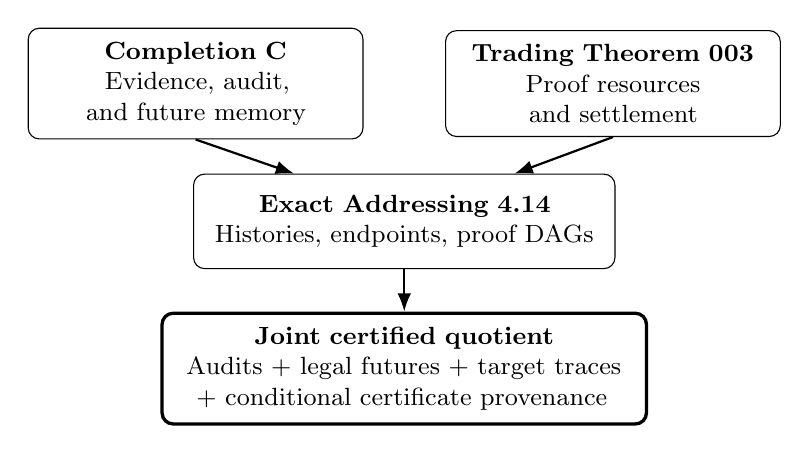
\begin{tikzpicture}[>=Latex,font=\small,b/.style={draw,rounded corners,align=center,inner sep=5pt,minimum height=12mm}]
\node[b,text width=3.9cm] (c) at (0,0) {\textbf{Completion C}\\Evidence, audit, and future memory};
\node[b,text width=3.9cm] (t) at (5.3,0) {\textbf{Trading Theorem 003}\\Proof resources and settlement};
\node[b,text width=5cm] (e) at (2.65,-1.75) {\textbf{Exact Addressing 4.14}\\Histories, endpoints, proof DAGs};
\node[b,very thick,text width=5.8cm] (j) at (2.65,-3.62) {\textbf{Joint certified quotient}\\Audits + legal futures + target traces\\+ conditional certificate provenance};
\draw[->,thick] (c.south)--([xshift=-1.4cm]e.north);
\draw[->,thick] (t.south)--([xshift=1.4cm]e.north);
\draw[->,thick] (e)--(j);
\end{tikzpicture}
\caption{The two conservation problems acquire a common domain through exact-addressed history and proof geometry. The arrows denote a proposed combination of obligations, not unconditional implications between manuscripts.}
\label{fig:integrated-spine}
\end{figure}

\paragraph{Provenance and methodological limits.} The evidence-calculus material below comes from Completion C and its A/B ancestors. History unfolding, annotated coterminal proof structures, extraction and cost-preserving bisimulation come from the Exact Addressing prologue. The resource-trading and settlement-search interpretations come from Trading Theorem 003. The endpoint and joint results are derived applications presented with proofs. This does not assert absolute mathematical novelty or a formally certified performance improvement.
\section{Frozen protocol and the audit interface}
Fix the inherited environment
\[
M=(\Gamma,F,V,O_T,O_R,P^*,A,\tau,L,c),
\]
where $F$ and $\Gamma$ are the fixed proof calculus and hypotheses; $V$ is a total decidable finite-proof verifier; $A$ is a fixed total decidable authentication, scope, and ancestry policy; $\tau$ is a fixed decidable trust policy; $L$ is a typed append-only finite event ledger at each finite time; and $c$ assigns finite nonnegative rational event charges. The original BANK is immutable and distinct from the proof-event ledger. Only a successful check by $V$ permits proof-event admission. The ideal source answers $H(e)$ correctly by semantic stipulation; that stipulation is not a computable implementation.

\begin{definition}[Admissible finite history]
For this paper a \emph{history} $h$ is a finite, locally closed accepted snapshot, including its finite registered-formula roster, complete accessible payloads and proof objects, finite acyclic ancestry chains, validation data, and the versions and locally executable inputs for $V,A,\tau$. Let $\Hh$ be a stated family of such histories within one fixed protocol profile. Unless otherwise specified, $\Hh$ is the family of syntactically admissible histories under the fixed local acceptance rules; it does \emph{not} require a decision procedure for semantic truth of all oracle assertions. A subclass $\Hh_{\rm true}$ may additionally satisfy the ideal source-truth contract.
\end{definition}

The receiver does not infer unrecorded physical events from a locally closed snapshot. In particular, a pointer whose target disappears with $O_T$ does not constitute a closed witness. The distinction between syntactic acceptance and semantic truth is necessary to avoid silently assuming a halting decider when reasoning about finite records.

\begin{definition}[Typed evidence view]
For each registered effectively encoded sentence $\varphi$, define
\begin{align*}
E_h(\varphi)&=(p_h(\varphi),a_h(\varphi),r_h(\varphi),u(\varphi))\in\{0,1\}^4,\\
p_h(\varphi)&=1\ \Longleftrightarrow\ \exists\pi\text{ in the proof ledger with }V(\pi,\Gamma,\varphi)=1,\\
a_h(\varphi)&=1\ \Longleftrightarrow\ \exists\text{ accepted origin receipt asserting }\varphi,\\
r_h(\varphi)&=1\ \Longleftrightarrow\ \exists\text{ accepted }O_T\to O_R\to P^*\text{ chain asserting }\varphi,\\
u(\varphi)&=1\ \Longleftrightarrow\ \Tr_\tau(O_T,\varphi).
\end{align*}
The inherited policy-relative admission bit is
\[
K_h^\tau(\varphi)=p_h(\varphi)\lor(a_h(\varphi)\land u(\varphi)).
\]
The witness bundle $W_h(\varphi)$ comprises the finite recorded matching proof certificates, origin records, accepted relay chains, and the applicable trust-policy entry. Transport alone cannot add a verified proof. As in A and B, the relay flag is displayed separately rather than being made an extra conjunct in the frozen admission rule.
\end{definition}

\begin{definition}[Authorized retrospective audit]
An \emph{audit interface} $Q:\Hh\to\Obs$ sends each admissible history to a finite, effectively encoded answer to an explicitly stated finite set of questions. The \emph{full finite-roster audit} $Q_{\rm full}$ serializes, in a fixed canonical order, the registered roster and the pairs
\[
\bigl(E_h(\varphi),W_h(\varphi)\bigr)
\quad\text{for each registered }\varphi.
\]
Canonical ordering and finite encodings are fixed in advance. Where witness equivalence rather than byte-for-byte identity is intended, it must be a declared, decidable equivalence with an effective canonical representative for each encountered finite witness object. The corresponding $Q$ records those representatives. A \emph{restricted audit}, such as $Q_K$, may ask only for the admission bits on a fixed roster.
\end{definition}

The object $Q_{\rm full}(h)$ is computable from a locally closed finite $h$: scan the finite proof and message projections, invoke total local checkers, enumerate matching finite witnesses, and serialize the result. This is a \emph{finite-record} computation, not a method for resolving the truth of arbitrary arithmetic statements. For comparisons, either use a common fixed roster or include each varying roster in the audit output.

\begin{figure}[htbp]\centering
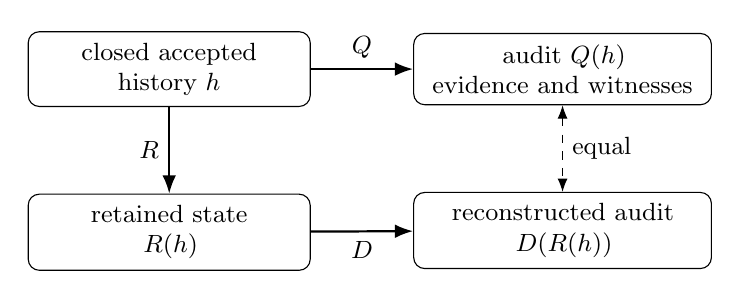
\begin{tikzpicture}[>=Latex,every node/.style={font=\small},b/.style={draw,rounded corners,align=center,minimum height=9mm,inner sep=4pt}]
\node[b,text width=3.3cm] (h) {closed accepted\\history $h$};
\node[b,right=13mm of h,text width=3.5cm] (q) {audit $Q(h)$\\evidence and witnesses};
\draw[->,thick] (h) -- node[above]{$Q$} (q);
\node[b,below=11mm of h,text width=3.3cm] (r) {retained state\\$R(h)$};
\node[b,below=11mm of q,text width=3.5cm] (d) {reconstructed audit\\$D(R(h))$};
\draw[->,thick] (h)--node[left]{$R$}(r);
\draw[->,thick] (r)--node[below]{$D$}(d);
\draw[<->,dashed] (q)--node[right]{equal}(d);
\end{tikzpicture}
\caption{Retrospective sufficiency asks whether the two paths return identical authorized audit answers. It does not require reproduction of every unasked historical fact.}
\label{fig:factor}
\end{figure}

\section{The geometry: history trees, endpoints, and proof objects}\label{sec:geometry}
The evidence ledger does not exhaust the geometry of an ATP. A single state may be reached by many different sequences of choices, failed attempts, or cached-proof retrievals. An accepted proof object is not even the same kind of mathematical object as an execution history. We formalize these differences before constructing a state quotient.

\begin{definition}[Labeled ATP and finite-history unfolding]
Fix a modeled labeled transition system $\mathbb A=(S,s_0,M,\longrightarrow,\operatorname{Obs})$. The complete states include the data declared relevant to legal futures, including verifier scope, receipt records, budgets, scheduler choices and authorizations when those are modeled. A \emph{finite execution history} is a represented sequence
\[
h=(s_0,a_1,s_1,\ldots,a_k,s_k),\qquad s_{j-1}\mathrel{\xrightarrow{a_j}}s_j.
\]
Its \emph{endpoint} is $e(h)=s_k$. Let $\Hh_{\rm exec}$ consist of all finite legal histories from $s_0$. An edge $h\to h'$ in the \emph{history unfolding} appends exactly one legal labeled step. The finite execution history $h$ and an accepted ledger snapshot are different types of objects. A declared readout map $\lambda:\Hh_{\rm exec}^{\rm aud}\to\Hh$ associates an audit-bearing execution history with its locally closed accepted evidence snapshot; the readout need not be injective and need not be defined on every legal run. For any ledger audit $Q_{\rm led}:\Hh\to\Obs$ the corresponding execution-history audit is $Q_{\rm exec}=Q_{\rm led}\circ\lambda$ on the declared domain. One may also explicitly declare a trace-sensitive audit that reads the entire represented history rather than only $\lambda(h)$. We do not identify these types or domains without specifying the readout.
\end{definition}

\begin{proposition}[History coverage and the many-to-one endpoint map]\label{prop:unfold}
The finite-history unfolding is a rooted directed tree, possibly infinite, with unique predecessor obtained by deleting a final step. Every finite legal state path corresponds to a unique root-to-history path. The endpoint projection $e$ maps onto the reachable operational states, but is generally not injective.
\end{proposition}
\begin{proof}
Deleting the final step is the unique predecessor of a nonempty finite represented sequence. Each deletion decreases length, ruling out cycles and guaranteeing eventual arrival at the empty history. Conversely, extension by legal steps yields the represented path, so all finite legal histories appear. The endpoint of a legal history is reachable, and every reachable state has a finite witnessing history. Distinct histories may share one endpoint when paths merge or a state is revisited.
\end{proof}

\begin{figure}[htbp]\centering
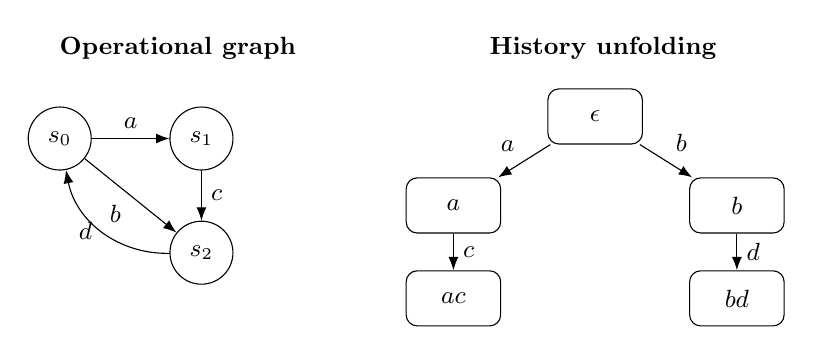
\begin{tikzpicture}[>=Latex,font=\small,b/.style={draw,circle,minimum size=8mm,inner sep=1pt},hb/.style={draw,rounded corners,minimum width=12mm,minimum height=7mm}]
\node[font=\small\bfseries] at (-2.7,1.75) {Operational graph};
\node[b] (s0) at (-4.2,.6) {$s_0$}; \node[b] (s1) at (-2.4,.6) {$s_1$};\node[b] (s2) at (-2.4,-.85) {$s_2$};
\draw[->] (s0)--node[above]{$a$}(s1);\draw[->] (s0)--node[below left]{$b$}(s2);\draw[->] (s1)--node[right]{$c$}(s2);\draw[->,bend left=40] (s2) to node[left]{$d$}(s0);
\node[font=\small\bfseries] at (2.7,1.75) {History unfolding};
\node[hb] (r) at (2.6,.88) {$\epsilon$};\node[hb] (aa) at (.8,-.25) {$a$};\node[hb] (bb) at (4.4,-.25) {$b$};\node[hb] (ac) at (.8,-1.43) {$ac$};\node[hb] (bd) at (4.4,-1.43) {$bd$};
\draw[->] (r)--node[above left]{$a$}(aa);\draw[->] (r)--node[above right]{$b$}(bb);\draw[->] (aa)--node[right]{$c$}(ac);\draw[->] (bb)--node[right]{$d$}(bd);
\end{tikzpicture}
\caption{An operational graph may revisit a state, while the unfolded history tree never identifies two different prefixes. The displayed tree is only a finite portion of the unfolding.}
\label{fig:history-geometry}
\end{figure}

\begin{definition}[Certified extraction and lineage]
For fixed $(F,\Gamma,V)$, let $\mathcal P_{F,\Gamma,V}$ denote the accepted, annotated terminally marked proof DAGs, with a designated terminal formula and checker scope. On a declared certified-history domain $\Hh_{\rm cert}\subseteq\Hh_{\rm exec}$, a partial computable extractor $E$ returns a candidate $D$ which the independent verifier accepts. A distinct checkable predicate $\mathsf{Origin}(h,D)$ states that the claimed proof ancestry is supported by event identifiers, scope, and receipt references. Neither checker acceptance nor a common theorem label entails $\mathsf{Origin}(h,D)$.
\end{definition}

Two runs can retrieve the same cached valid proof $D$ but have different origins. Conversely, two distinct verified DAGs may conclude the same theorem. Exact Addressing's coterminal proof geometry allows safe reversal of individually tagged proof DAGs, and gluing their designated backward roots, \emph{without} globally merging every vertex bearing the same formula. The latter operation may introduce cycles, erase premise ports, or confuse AND-premises with OR-alternatives.

\begin{figure}[htbp]\centering
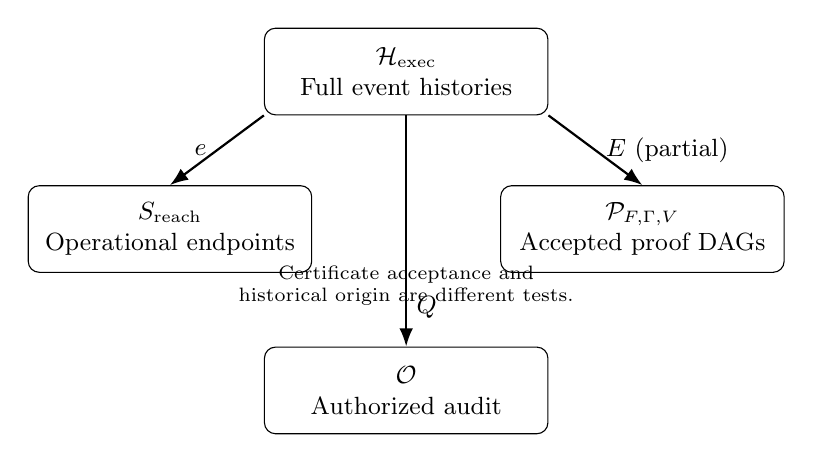
\begin{tikzpicture}[>=Latex,font=\small,b/.style={draw,rounded corners,align=center,inner sep=5pt,minimum width=36mm,minimum height=11mm}]
\node[b] (h) at (0,0) {$\mathcal H_{\rm exec}$\\Full event histories};
\node[b] (s) at (-3,-2) {$S_{\rm reach}$\\Operational endpoints};
\node[b] (p) at (3,-2) {$\mathcal P_{F,\Gamma,V}$\\Accepted proof DAGs};
\node[b] (a) at (0,-4.05) {$\Obs$\\Authorized audit};
\draw[->,thick] (h.south west)--node[left,pos=.5]{$e$}(s.north);
\draw[->,thick] (h.south east)--node[right,pos=.5]{$E$ (partial)}(p.north);
\draw[->,thick] (h.south)--node[right,pos=.83]{$Q$}(a.north);
\node[font=\scriptsize,align=center] at (0,-2.72) {Certificate acceptance and\\historical origin are different tests.};
\end{tikzpicture}
\caption{Histories, endpoints, and proof objects have different identities. Any audit quotient must specify which distinctions it is allowed to forget.}
\label{fig:three-spaces}
\end{figure}

\paragraph{Addresses versus quotients.} An injective address $\mathsf{addr}_{\Hh}(h)$ keeps individual histories distinct. A proof address $\mathsf{addr}_{\mathcal P}(D)$ keeps accepted DAG objects distinct. A quotient address $\mathsf{addr}_{\sim}([s])$, if effectively implemented, \emph{merges} selected states. These addresses are not interchangeable. A loss of historical identity can be intentional for settlement search and inadmissible for a provenance audit.

\section{The exact retrospective preservation theorem}
\begin{definition}[Retention and sufficiency]
A \emph{retention map} is a function $R:\Hh\to\State$, where $\State\subseteq\{0,1\}^*$ consists of finite stored representations. It is \emph{$Q$-sufficient} if some reconstruction function $D:R[\Hh]\to\Obs$ satisfies
\[
D(R(h))=Q(h)\quad\text{for every }h\in\Hh.
\]
The requirement is exact equality of authorized audit outputs, not reconstruction of the entire physical execution. No effectiveness or efficiency of $D$ is presupposed in this definition.
\end{definition}

\begin{theorem}[Exact retrospective preservation criterion]\label{thm:static}
A retention map $R$ is $Q$-sufficient if and only if
\begin{equation}\label{eq:kernel}
\forall h_1,h_2\in\Hh,\quad R(h_1)=R(h_2)\ \Longrightarrow\ Q(h_1)=Q(h_2).
\end{equation}
In other words, $\ker(R)\subseteq\ker(Q)$, where $\ker(f)$ denotes equality of outputs under $f$.
\end{theorem}
\begin{proof}
Suppose $Q=D\circ R$. If $R(h_1)=R(h_2)$, applying $D$ to both sides gives $Q(h_1)=Q(h_2)$. Conversely, suppose (\ref{eq:kernel}) holds. For any reachable retained value $s\in R[\Hh]$, choose any $h\in\Hh$ with $R(h)=s$ and set $D(s)=Q(h)$. The hypothesis makes the value independent of the chosen representative. Thus $D$ is a well-defined function on the reachable range and $D(R(h))=Q(h)$ for every $h$.
\end{proof}

The converse is deliberately \emph{extensional}: making $D$ well defined does not, by itself, produce even an executable decoder, let alone an efficient one. The following result states a separate sufficient effectiveness condition.

\begin{proposition}[Effective reconstruction on an enumerable domain]\label{prop:effective}
If $\Hh$ has a computable enumeration of its valid finite encodings, $Q$ and $R$ are total computable on those encodings, and (\ref{eq:kernel}) holds, then a partial computable $D$ exists which halts and gives the correct audit on every $s\in R[\Hh]$. No claim is made that membership in $R[\Hh]$ is decidable or that the search is efficient.
\end{proposition}
\begin{proof}
Given $s$, enumerate $h\in\Hh$ until finding one with $R(h)=s$, then output $Q(h)$. Equality of the finite retained encodings is decidable. On every reachable $s$ a preimage eventually appears, so this procedure halts. Equation (\ref{eq:kernel}) makes the result independent of which matching history is first enumerated.
\end{proof}

\begin{remark}[The oracle-truth trap]
Syntactically accepted finite transcripts can be enumerated under a decidable local profile; a family restricted by the requirement that every oracle bit equal the true halting predicate need not be effectively enumerable in the same way. Proposition \ref{prop:effective} is therefore conditional on its stated effective-domain hypothesis, and must not be invoked silently for the oracle-truthful subclass.
\end{remark}


\begin{example}[Extensional sufficiency without any computable decoder]\label{ex:truth-obstruction}
Fix a protocol instance whose decidable syntactic origin policy permits well-formed finite bit receipts. Consider the mathematical family
\[
\Hh_{\rm true}^{\rm bit}=\{h_e=\mathsf{pad}(e,H(e)):e\text{ a standard machine/input code}\},
\]
where $H(e)$ is supplied by the \emph{ideal truthful source}, not computed locally. Here $\mathsf{pad}$ is a fixed computable encoding that embeds an arbitrary finite pair $(e,b)$ in a complete locally closed, syntactically accepted origin-receipt history under this illustrative admissible profile; the other required administrative and checker fields are computably supplied by the fixed profile. This explicitly assumes a profile with a computable syntactic receipt-template constructor, and does not assume that its assertions are semantically true. On the truthful subclass let
\[
R(\mathsf{pad}(e,b))=e,\qquad Q(\mathsf{pad}(e,b))=b.
\]
Both maps are computable projections of the \emph{presented finite records}. Because the truthful family contains exactly one bit for each $e$, $R(h_e)=R(h_f)$ implies $Q(h_e)=Q(h_f)$. Thus Theorem \ref{thm:static} yields a set-theoretic decoder $D(e)=H(e)$. There is nevertheless no ordinary computable decoder on all reachable codes, by the diagonal halting argument. This is not a valid invocation of Proposition \ref{prop:effective}: a computable enumeration of all truthful pairs $(e,H(e))$ would itself compute $H$, by waiting for the enumerated pair with the requested $e$. The example concerns an ideal-source semantic subclass and does not manufacture an executable oracle. In particular, locally closed \emph{stored} original receipts can be audited computably, but deleting the relevant bits destroys this effective guarantee.
\end{example}

\begin{definition}[Effective $Q$-sufficiency]\label{def:effective}
For a stated represented domain, a retention map is \emph{effectively $Q$-sufficient} if an explicitly specified partial computable decoder $D$ halts with $D(R(h))=Q(h)$ on every reachable retained state. A prospective representation is \emph{effectively prospectively sufficient} when its audit decoder, enabled-action test, and retained transition are all partial computable and halt on every permitted reachable input. These are stronger requirements than existence of abstract functions; an algorithm or adequate additional computability hypotheses must be supplied.
\end{definition}

\begin{definition}[Audit equivalence]
Write $h\equiv_Q h'$ if and only if $Q(h)=Q(h')$. Let $[h]_Q$ denote its equivalence class. The quotient map $q_Q:h\mapsto[h]_Q$ is the \emph{canonical observational quotient} associated with the chosen retrospective audit.
\end{definition}

\begin{corollary}[Coarsest sufficient partition]\label{cor:quotient}
The quotient map $q_Q$ is $Q$-sufficient, and every $Q$-sufficient retention map distinguishes at least the pairs distinguished by $q_Q$. Thus $\equiv_Q$ is the coarsest permissible equality-of-retained-state relation for retrospective sufficiency.
\end{corollary}
\begin{proof}
The audit is constant on each $Q$-equivalence class by definition, so Theorem \ref{thm:static} applies to $q_Q$. Any other sufficient $R$ obeys $\ker(R)\subseteq\ker(Q)$ by that theorem.
\end{proof}

This is a mathematical minimality result about \emph{which distinctions must be retained}. It is not a shortest-program theorem, a claim about physical storage optimality, or a unique byte encoding. In a computable finite-record setting $Q(h)$ itself is one canonical sufficient \emph{retrospective} stored output, although computing or maintaining it may be costly and it need not support later updates.

\section{When an operational endpoint is enough}\label{sec:endpoint}
The endpoint map from Section \ref{sec:geometry} is the first candidate retention scheme: keep the complete operational state but erase the path that led to it. The audit in the following theorem is any \emph{declared} execution-history audit, for example $Q_{\rm led}\circ\lambda$ on a compatible audit-bearing domain. When the domain is restricted, we require it to contain an endpoint witness for each state called reachable below. The exact retrospective theorem supplies a necessary and sufficient test.

\begin{theorem}[Endpoint sufficiency criterion]\label{thm:endpoint}
Let $Q:\Hh_{\rm exec}\to\Obs$ be a declared audit on the full modeled execution-history space, and let $e:\Hh_{\rm exec}\to S_{\rm reach}$ be the endpoint projection. (An audit defined only on a restricted domain has the analogous statement with its endpoint image in place of $S_{\rm reach}$.) There exists a function $\widehat Q:S_{\rm reach}\to\Obs$ with $Q=\widehat Q\circ e$ if and only if
\[
e(h)=e(h')\quad\Longrightarrow\quad Q(h)=Q(h')
\qquad\text{for all }h,h'\in\Hh_{\rm exec}.
\]
No effective decoder is implied without separate hypotheses.
\end{theorem}
\begin{proof}
Use Theorem \ref{thm:static} with retention $R=e$, restricting its history domain to $\Hh_{\rm exec}$. The forward implication follows by applying $\widehat Q$ to equal endpoints. For the converse, assign to each reachable state $s$ the value $Q(h)$ of any history ending at $s$; the condition makes this assignment independent of the selected history.
\end{proof}

The theorem is modest as an abstract result and decisive as a diagnostic test. If two histories with distinct audited receipts have one final state, that state was too small to serve as the archive; quotienting it again cannot repair the loss. Options include enriching the operational state with the required receipt distinction, narrowing the advertised audit, or retaining an auxiliary history address. A complete state as modeled in Exact Addressing normally includes whatever the system has \emph{declared} necessary for future behavior, but this is not by itself a promise to preserve every retrospective origin question a later observer might ask.

\begin{corollary}[A two-stage quotient audit test]\label{cor:two-stage}
Assume the endpoint criterion and let $q:S_{\rm reach}\to\mathcal Z$ be any second retention map. Then the history audit can be recovered abstractly from $q\circ e$ precisely when
\[
q(s)=q(t)\ \Longrightarrow\ \widehat Q(s)=\widehat Q(t)
\qquad(s,t\in S_{\rm reach}).
\]
\end{corollary}
\begin{proof}
The displayed condition is sufficient by factoring $\widehat Q$ through $q$ and composing the decoder with $e$. It is necessary because every reachable $s,t$ have endpoint witnesses $h,h'$, so equality of retained class codes must imply equality of their audit results.
\end{proof}

\paragraph{Computability is an additional gate.} Even if $e$ and $q$ can be evaluated on individual finite histories, the abstract factorization may lack an executable decoder on a semantic truthful-oracle subclass. Example \ref{ex:truth-obstruction} is a direct witness. The effective tests in Definition \ref{def:effective} remain prerequisites for claiming a functioning Pioneer archive.

\section{Why admission alone loses epistemic history}
\begin{example}[One admitted proposition, two distinct warrants]\label{ex:proof-vs-att}
Fix a registered sentence $\varphi$ for which $V$ accepts a genuine finite proof from $\Gamma$, and suppose the trusted source can issue an $A$-accepted receipt asserting the same true $\varphi$. A simple instance is a decidably halting machine's correctly encoded halting claim, provided the fixed formal profile admits the indicated proof and receipt. Consider locally closed histories $h_p$ and $h_a$ on the same roster with the same frozen trust flag $u(\varphi)=1$:
\[
\begin{array}{c|cccc|c}
& p&a&r&u&K^\tau\\\hline
h_p&1&0&0&1&1\\
h_a&0&1&1&1&1
\end{array}
\]
The first retains a verifier-accepted proof; the second retains an accepted trusted source receipt and two-hop path, but no proof. Both are admitted under the inherited rule, so $Q_K(h_p)=Q_K(h_a)$ for the one-sentence admission-only audit. However, $Q_{\rm full}(h_p)\ne Q_{\rm full}(h_a)$. A compression that stores only $K^\tau$ is sufficient for the first restricted question and insufficient for the second, richer interface.
\end{example}

\begin{proposition}[Witness sensitivity]\label{prop:witness}
If an audit requires the complete finite accepted witness bundle, then two histories that have the same evidence vector but different required witness encodings cannot be merged by a sufficient retention map. If the audit requires witnesses only up to a declared effective equivalence, it may merge histories whose normalized witness bundles agree.
\end{proposition}
\begin{proof}
In the first case the audit outputs differ because their required witness components differ, so Theorem \ref{thm:static} prohibits equal retention. In the second case normalization makes the respective witness components equal, and there is no obstruction from those components; other audit fields must still agree.
\end{proof}

\begin{remark}[Authenticity is not truth]
These examples distinguish an accepted origin claim from a verified proof without inferring mathematical truth from a signature. A statement admitted via $a\land u$ is sound only if the trusted source assertions are in fact correct; a statement admitted via $p$ requires the intended soundness of $V$ and $\Gamma$. The verifier firewall remains unchanged.
\end{remark}


\section{The proof may survive while its origin disappears}\label{sec:proof-origin}
A settlement-only audit might return just the answer $\mathbf 1_{T}(s)$ or the existence of a $V$-accepted proof. A stronger audit may require the certificate bytes, scope, or an \emph{origin witness} tying that proof to a specific history. These are distinct informational demands. The following example is intentionally elementary.

\begin{example}[One valid cached proof, two different origins]
Let histories $h_1,h_2$ both end with the same accepted proof object $D$ of $\varphi$. In $h_1$ the preceding event record includes the steps and identifiers to substantiate $\mathsf{Origin}(h_1,D)$. In $h_2$ the same $D$ is obtained by retrieving a cache entry, but no record substantiates a claim that this execution itself generated $D$. Checker acceptance agrees in both histories. If the origin audit reports whether the respective claimed lineage is substantiated, then its outputs differ. Thus no retention map identifying $h_1$ and $h_2$ can be sufficient for that origin audit, even if a theorem-only audit merges them safely.
\end{example}

\begin{proposition}[Proof extraction is not enough for lineage preservation]\label{prop:origin-factor}
Suppose $E(h)=D$ is defined and verifier accepted on the certified-history domain, and $Q_{\rm orig}(h)$ is a specified origin-audit output. A decoder using \emph{only} the extracted proof $E(h)$ exists if and only if
\[
E(h)=E(h')\implies Q_{\rm orig}(h)=Q_{\rm orig}(h')
\]
for all certified histories in that domain. In particular, checker acceptance alone does not imply the factorization.
\end{proposition}
\begin{proof}
Apply Theorem \ref{thm:static} to $R=E$ on its certified domain. The preceding example shows that accepting the same proof does not force equality of origin-audit outputs.
\end{proof}

\begin{figure}[htbp]\centering
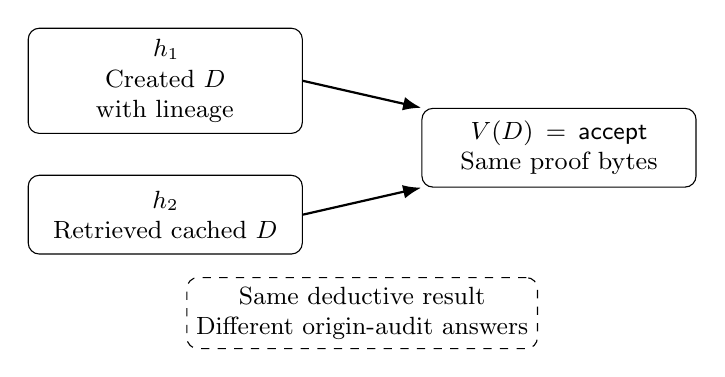
\begin{tikzpicture}[>=Latex,font=\small,b/.style={draw,rounded corners,minimum height=10mm,align=center,inner sep=4pt}]
\node[b,text width=3.2cm] (one) at (0,.85) {$h_1$\\Created $D$ with lineage};
\node[b,text width=3.2cm] (two) at (0,-.85) {$h_2$\\Retrieved cached $D$};
\node[b,text width=3.2cm] (proof) at (5,0) {$V(D)=\mathsf{accept}$\\Same proof bytes};
\draw[->,thick] (one.east)--(proof.north west);
\draw[->,thick] (two.east)--(proof.south west);
\node[draw,dashed,rounded corners,align=center,font=\small] at (2.5,-2.1) {Same deductive result\\Different origin-audit answers};
\end{tikzpicture}
\caption{Proof certification survives both histories, but the stronger claim of having generated the proof requires independently retained lineage records.}
\label{fig:origin-split}
\end{figure}

This example explains why exact addressing of proof DAGs is distinct from exact addressing of histories. A memory system may reasonably retain a single shared proof object with compact, separately checkable origin pointers for each run. That is a proposed architecture, not a proven cost saving: the validity of those pointers and their checking charges must be established in a specified implementation.

\section{A worked oracle-ledger compression and a future-action obstruction}\label{sec:worked}
The next construction makes the synergy operational in one deliberately narrow, frozen protocol \emph{instance}. It is a mathematical example of a constrained accepted-ledger family, not a modification to the inherited engine or a claim of universal source-trace compression.

\begin{example}[A two-bit continuing archive for an unbounded ledger family]\label{ex:concrete-ledger}
Fix a decidable authentication/ancestry policy $A$, fixed trust policy $\tau$, and the unchanged verifier gate $V$ satisfying the inherited type separation. Choose a true, registered halting-bit sentence $\varphi\equiv H(e_*)=1$, where $e_*$ is a specified immediately halting code, with $\tau$ trusting the source for $\varphi$. Fix two distinct, accepted, source-authenticated receipt templates $r_0,r_1$ asserting $\varphi$, with distinct query identifiers $q_0,q_1$ and complete finite validation data. The templates may be generated by a finite lookup table; their acceptance is part of the stated finite instance of the frozen profile. Also choose an unrelated true sentence $\psi\equiv H(e_\infty)=0$ for an explicitly looping machine, and permit an arbitrary finite number $n$ of distinct, locally closed, source-authenticated $\psi$-records, none addressed by the actions below. Only finitely many ideal truthful oracle answers (issued before any source deactivation) are used; no local algorithm is required to solve halting. This illustration allows multiple original queries, while the inherited basic preservation theorem needs only one.

For $i,t\in\{0,1\}$ and $n\in\N$, let $h_{i,n,t}$ be a finite locally closed accepted ledger with exactly one $\varphi$-origin record $r_i$, those $n$ auxiliary $\psi$-records, no accepted $\varphi$-proof, and (if $t=1$) exactly one correctly validated two-hop relay chain for $r_i$. If $t=0$, there is no completed $\varphi$-path. All ancestor bytes, independent checker data, and fixed policy versions required for these records remain locally available. The restricted audit asks \emph{only} for the four evidence bits of $\varphi$, not costs, message counts, $\psi$-witnesses, or full provenance:
\[
Q_{\varphi}(h_{i,n,t})=(p,a,r,u)=(0,1,t,1),
\qquad K^\tau(\varphi)=1.
\]
There are infinitely many distinct ledgers because the $\psi$-records have distinct finite identifiers, but the authorized audit has only two outputs. The one-bit retrospective retention
\[
R_{\rm now}(h_{i,n,t})=t,\qquad D_{\rm now}(t)=(0,1,t,1)
\]
is explicitly computable and $Q_{\varphi}$-sufficient, uniformly in $n$.

To model a continuing Pioneer, restrict the action alphabet to $\{\mathsf{deliver}(0),\mathsf{deliver}(1)\}$. The action $\mathsf{deliver}(j)$ is enabled \emph{exactly} when $t=0$ and $i=j$; it appends the correctly authenticated two-hop chain referencing $r_j$ and changes $t$ to $1$. No actions are enabled once $t=1$. The authorization and predecessor checks use the same fixed $A$ and the stored templates; the only supplied new object is the corresponding finite relay envelope. These are the \emph{declared} admissible future actions for this example, not every possible action of a general AMLD ledger.

Define a two-bit archive and explicit transition operations by
\[
R_{\rm cont}(h_{i,n,t})=(i,t),\quad D_{\rm cont}(i,t)=(0,1,t,1),
\]
\[
\mathsf{enabled}((i,t),\mathsf{deliver}(j))\iff (t=0\ \wedge\ i=j),
\]
\[
\bar\delta((i,0),\mathsf{deliver}(i))=(i,1).
\]
These finite algorithms exactly reproduce the audit, enabled actions, and successor retention for the entire family. They discard the unbounded number of auxiliary $\psi$-records and their histories. Thus they give an explicit, nontrivial, \emph{effectively prospectively sufficient} compression for this restricted interface and action set, without changing the proof BANK or allowing a message to enter the proof ledger.
\end{example}

\begin{proposition}[A retained admission or relay flag is insufficient for continuation]\label{prop:concrete-obstruction}
In Example \ref{ex:concrete-ledger}, $R_{\rm now}$ is not prospectively sufficient for the stated two-action transition system. The two-bit map $R_{\rm cont}$ is effectively prospectively sufficient, although it is not claimed to be the coarsest possible encoding.
\end{proposition}
\begin{proof}
The two states $h_{0,0,0}$ and $h_{1,0,0}$ have equal current audit and equal $R_{\rm now}$ value $0$, but $\mathsf{deliver}(0)$ is enabled only in the first. Hence the kernel of $R_{\rm now}$ fails the enabled-action condition of a $Q$-congruence. For $R_{\rm cont}$, equal pairs $(i,t)$ have identical audits and enabled actions. Any enabled delivery maps them to pairs $(i,1)$ independent of $n$. The displayed explicit computable decoder and updater therefore satisfy the stronger effective prospective requirement of Definition \ref{def:effective}.
\end{proof}

\begin{remark}[Exact scope of the compression claim]
This is an improvement in retained-state \emph{size} only when the task deliberately excludes ancillary $\psi$ evidence and costs and prohibits future actions addressing those deleted records. The two-bit archive does \emph{not} preserve $Q_{\rm full}$ on a roster containing $\psi$, the complete witness bundle, all historical charges, arbitrary future reference links, or unrestricted revalidation. Such broader audit requirements can force the discarded records to remain. Any implementation must still account for fixed authentication code, template tables, and the cost of reconstructing or supplying a relay envelope; none of these hidden resources is declared free.
\end{remark}

\begin{figure}[htbp]\centering
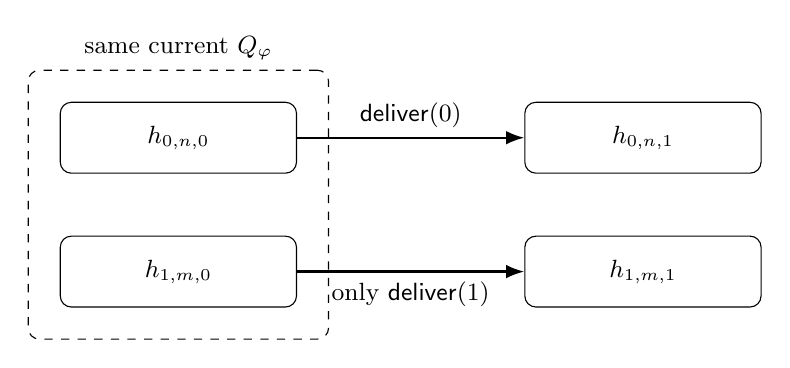
\begin{tikzpicture}[>=Latex, every node/.style={font=\small}, b/.style={draw,rounded corners,align=center,minimum height=9mm,minimum width=30mm,inner sep=4pt}]
\node[b] (a) at (0,0.85) {$h_{0,n,0}$};
\node[b] (b) at (0,-0.85) {$h_{1,m,0}$};
\node[b] (ar) at (5.9,0.85) {$h_{0,n,1}$};
\node[b] (br) at (5.9,-0.85) {$h_{1,m,1}$};
\node[draw,dashed,rounded corners,fit=(a)(b),inner sep=4mm,label=above:{same current $Q_\varphi$}] {};
\draw[->,thick] (a.east)--node[above]{$\mathsf{deliver}(0)$}(ar.west);
\draw[->,thick] (b.east)--node[below]{only $\mathsf{deliver}(1)$}(br.west);
\end{tikzpicture}
\caption{The restricted current audit forgets the receipt ID. A future authenticated predecessor check must still distinguish the two histories. The auxiliary record counts $n,m$ need not survive under this restricted action alphabet.}
\label{fig:worked}
\end{figure}

\section{An information lower bound for finite archival families}
\begin{theorem}[Finite distinguishability bound]\label{thm:bits}
Let $T\subseteq\Hh$ be a nonempty finite family of histories, and put
\[
N=\bigl|\{Q(h):h\in T\}\bigr|.
\]
If $R$ is $Q$-sufficient on $T$, then $\bigl|R[T]\bigr|\ge N$. Consequently, any fixed-length $b$-bit encoding of retained states on $T$ satisfies
\[
b\ \ge\ \left\lceil\log_2 N\right\rceil.
\]
For this \emph{finite specified family} the cardinality bound is achievable by assigning a distinct binary label to each audit-equivalence class; this asserts no uniform or efficient compressor for unbounded history families.
\end{theorem}
\begin{proof}
Choose one history from each of the $N$ distinct audit classes in $T$. By Theorem \ref{thm:static}, no two selected histories can share an $R$-value. Thus at least $N$ distinct retained values are required. There are at most $2^b$ binary strings of length $b$, hence $2^b\ge N$. For attainability on the given finite family, assign distinct labels of length $\lceil\log_2 N\rceil$ to the $N$ classes and use their common audit outputs to define the decoder.
\end{proof}

\begin{example}[Two questions can require more than one flag]
For a one-sentence roster, the restricted interface $Q_K$ has at most two outcomes, so the counting bound alone gives at most one required bit. An interface returning the separate proof, attestation, and relay flags can exhibit more outcomes under a suitable protocol family; each actually realized, distinct evidence pattern contributes another required audit class. Recording the complete witness bundle may yield many more classes even when the Boolean evidence vector is identical.
\end{example}

\paragraph{Cost qualification.} The lower bound measures only the distinguishability of audit outcomes within a fixed finite family. It is not a lower bound on the entire operational memory, on reconstructing all proof or provenance witnesses, or on the minimal time/space needed to maintain a continuing ATP. A coding achieving the bit count may depend on a family-specific lookup table. Variable-length descriptions, expected length under a distribution, storage of checking and decoding code, communication, authentication data, CPU time, and cost charges require separately declared models. The event ledger's finite rational charges make recorded sums computable but do not assign a physical cost to the ideal noncomputable oracle. No optimal compression ratio is claimed.

\section{Continuing agents need more than retrospective sufficiency}
Suppose the Pioneer must process new proof objects, receipts, and relay envelopes after the archive is formed. An answer-preserving snapshot is not necessarily a sufficient \emph{state} for these operations.

\begin{definition}[Deterministic audit transition system]\label{def:trans}
An \emph{audit transition system} is $(\Hh,\Act,\delta,Q)$, where $\Act$ is a specified set of finite action labels and $\delta:\Hh\times\Act\rightharpoonup\Hh$ is a deterministic partial transition map. Definedness means that the action is enabled and its finite accepted successor exists. In an instantiated frozen protocol, actions may represent locally checkable admission or storage steps, with externally supplied payloads named in the action labels. This abstraction neither inserts an oracle query into a computable local transition nor changes the inherited BANK, $V$, $A$, or $\tau$.
\end{definition}

\begin{definition}[$Q$-congruence]
An equivalence relation $\sim$ on $\Hh$ is a \emph{$Q$-congruence} if, whenever $h\sim h'$, (i) $Q(h)=Q(h')$; (ii) for every $a\in\Act$, $\delta(h,a)$ is defined exactly when $\delta(h',a)$ is defined; and (iii) if they are defined, $\delta(h,a)\sim\delta(h',a)$.
\end{definition}

\begin{theorem}[Exact prospective preservation criterion]\label{thm:dynamic}
Let $R:\Hh\to\State$ be a retention map. The following are equivalent:
\begin{enumerate}[label=(\roman*)]
\item There exist well-defined deterministic functions on reachable retained states: a decoder $D$ satisfying $D(R(h))=Q(h)$, an enabled-action predicate agreeing with definedness of $\delta$, and a retained-state successor $\bar\delta$ satisfying $\bar\delta(R(h),a)=R(\delta(h,a))$ whenever the action is enabled.
\item The equivalence relation $\ker(R)$ is a $Q$-congruence.
\end{enumerate}
Consequently, under these conditions the quotient system produces the same audit outputs after every finite action sequence that is enabled from its starting history.
\end{theorem}
\begin{proof}
Assume (i). Equal retained states have equal decoded observations and the same enabled actions; applying the common retained-state successor to either representation gives equal retained successors. These are precisely the three clauses of a $Q$-congruence. Conversely, assume (ii). On a reachable state $s=R(h)$ set $D(s)=Q(h)$, declare $a$ enabled iff $\delta(h,a)$ is defined, and when enabled set $\bar\delta(s,a)=R(\delta(h,a))$. The congruence clauses make all three assignments independent of the chosen representative. This proves (i). For any finite action sequence, induction on its length shows that enabledness agrees and the retained state after each step is the image under $R$ of the full-history state. Applying $D$ yields identical audit outputs at the end of each enabled prefix.
\end{proof}

\begin{figure}[htbp]\centering
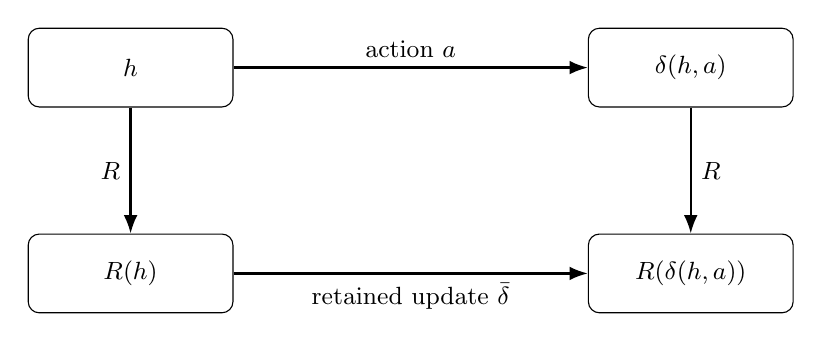
\begin{tikzpicture}[>=Latex,every node/.style={font=\small},b/.style={draw,rounded corners,minimum width=26mm,minimum height=10mm,align=center}]
\node[b] (h) {$h$};
\node[b,right=45mm of h] (ha) {$\delta(h,a)$};
\node[b,below=16mm of h] (rh) {$R(h)$};
\node[b,below=16mm of ha] (rha) {$R(\delta(h,a))$};
\draw[->,thick] (h)--node[above]{action $a$}(ha);
\draw[->,thick] (h)--node[left]{$R$}(rh);
\draw[->,thick] (ha)--node[right]{$R$}(rha);
\draw[->,thick] (rh)--node[below]{retained update $\bar\delta$}(rha);
\end{tikzpicture}
\caption{Prospective preservation requires the retention map to commute with permitted future transitions, not only with today's audit.}
\label{fig:commute}
\end{figure}

\begin{example}[An archive that knows today's answer but cannot process tomorrow's input]
Consider finite histories $x_0,x_1$ with identical current audit output $Q(x_0)=Q(x_1)=0$, and a future action $a$ enabled in both, but with $Q(\delta(x_0,a))=0$ and $Q(\delta(x_1,a))=1$. Retention $R=Q$ is retrospectively sufficient. It is not prospectively sufficient: if $R(x_0)=R(x_1)$, a single deterministic update of that retained state cannot produce both required future answers. In a provenance application, the erased distinction could be validation data needed to judge a subsequently presented predecessor link. This is an abstract countermodel, not an assertion that the frozen A/B protocol implements these four states verbatim.
\end{example}

\begin{corollary}[Verifier-firewall preservation under a suitable audit]
Suppose the authorized audit explicitly includes the verified-proof flags and $\ker(R)$ is a $Q$-congruence for the unchanged protocol transitions. Then every quotient transition has the same displayed proof status as its full-history counterpart. In particular, a message-only transition cannot be represented as increasing the verified-proof flag if it does not do so in the source system.
\end{corollary}
\begin{proof}
By Theorem \ref{thm:dynamic}, the next quotient state decodes to the exact audit of the next full-history state. In the frozen protocol, message-only events leave the proof projection unchanged. Their verified-proof flags therefore remain unchanged in both audited views.
\end{proof}

\section{The coarsest future-observational distinction}
The previous theorem describes safe retained states by a congruence. It is natural to ask whether there is a canonical \emph{largest} such relation, analogous to the retrospective quotient $\equiv_Q$.

For a finite action word $w=a_1\cdots a_n$, let $\delta^*(h,w)$ denote the iterated successor if all actions are enabled, and be undefined otherwise. Put $\delta^*(h,\epsilon)=h$ for the empty word. Let $\bot$ be a fresh symbol not equal to any audit output.
\begin{definition}[Future observational equivalence]
Define
\[
h\equiv_{Q,\delta}^{+}h'
\quad\Longleftrightarrow\quad
\forall w\in\Act^*,\ 
\mathsf{sig}_{h}(w)=\mathsf{sig}_{h'}(w),
\]
where $\mathsf{sig}_h(w)=Q(\delta^*(h,w))$ if the iterated transition is defined, and $\mathsf{sig}_h(w)=\bot$ otherwise.
\end{definition}

\begin{theorem}[Canonical prospective quotient]\label{thm:future}
The relation $\equiv_{Q,\delta}^{+}$ is a $Q$-congruence. Every other $Q$-congruence is contained in it. Thus the quotient by $\equiv_{Q,\delta}^{+}$ is the coarsest \emph{mathematically exact} deterministic retained-state partition preserving every future audit and enabled-action distinction.
\end{theorem}
\begin{proof}
Equality of signatures for all words is an equivalence relation. Taking $w=\epsilon$ proves equality of current $Q$-outputs. For any action $a$, comparing signatures at the one-letter word $a$ proves that $a$ is enabled from both histories or from neither, since $\bot$ is distinct from every audit output. If $a$ is enabled, then for every word $w$ the signature after $a$ followed by $w$ is the signature of successor under $w$. Equality of the original signatures therefore gives $\delta(h,a)\equiv_{Q,\delta}^{+}\delta(h',a)$. Hence it is a congruence.

Conversely, let $\sim$ be any $Q$-congruence and suppose $h\sim h'$. Induction on the length of $w$ shows that either both runs under $w$ are undefined or both are defined with $\sim$-related final states. In the latter case their $Q$-outputs agree. Hence their signatures agree for all words, proving $h\equiv_{Q,\delta}^{+}h'$.
\end{proof}

\begin{corollary}[Retrospective versus prospective classes]
\[
\equiv_{Q,\delta}^{+}\ \subseteq\ \equiv_Q.
\]
The inclusion can be strict: equality of present audit answers need not imply equality under future action sequences.
\end{corollary}
\begin{proof}
The empty-word comparison gives the inclusion. Strictness is witnessed by the preceding example with $x_0,x_1$ and action $a$.
\end{proof}

This supplies a concrete answer to the distinction between an archive and a continuing agent. The coarsest safe \emph{historical} quotient is determined by present audit outputs; the coarsest safe \emph{operational} quotient is determined by all possible future audits. Neither quotient is automatically a physically cheapest representation.

\section{From prospective memory to a joint settlement quotient}\label{sec:joint}
Completion C's future-observational equivalence is tailored to deterministic actions and their authorized audit outputs. A general proof-search graph may instead be nondeterministic: a state can have several legal successors under one nominal step label. The Quotient Hunter in Trading Theorem 003 asks which such states can be merged while preserving target reachability. Exact Addressing P.4 provides strong sufficient conditions for preserving \emph{labeled, costed} traces, not just one Boolean answer.

\begin{definition}[Weighted settlement and audit system]
Let $G=(S,E,w)$ be a reachable directed state graph with target set $T\subseteq S$ and labels $a$ on edges. Write $s\xrightarrow{a,c}t$ for a legal primitive step of cost $c\ge0$. Fix an authorized state audit $q:S\to\Obs$ and a history audit $Q:\Hh_{\rm exec}\to\Obs$. The \emph{endpoint compatibility} requirement is $Q=q\circ e$. Equivalently, it requires the endpoint criterion from Theorem \ref{thm:endpoint} and an explicit choice $q=\widehat Q$. A costed settlement trace is the finite sequence of labels and primitive charges along a path reaching $T$; it is not the total cost of discovering that path.
\end{definition}

\begin{definition}[Joint audit--settlement bisimulation]
An equivalence relation $\sim$ on reachable $S$ is a \emph{joint bisimulation} for $(q,T)$ if, whenever $s\sim t$:
\begin{enumerate}[label=(\roman*)]
\item $q(s)=q(t)$ and $s\in T\iff t\in T$;
\item every $s\xrightarrow{a,c}s'$ has a matching $t\xrightarrow{a,c}t'$ with $s'\sim t'$;
\item the same matching condition holds with $s$ and $t$ exchanged.
\end{enumerate}
The quotient has a labeled, costed edge $[s]\xrightarrow{a,c}[u]$ whenever such an edge exists between some representatives. This existential definition alone does not imply path lifting; the matching conditions do the essential work.
\end{definition}

\begin{theorem}[Certified epistemic--settlement quotient theorem]\label{thm:joint}
Assume endpoint compatibility $Q=q\circ e$. If $\sim$ is a joint audit--settlement bisimulation, then the quotient $S/{\sim}$ has the following properties.
\begin{enumerate}[label=(\alph*)]
\item The history audit factors through the quotient endpoint: there is a unique function $\widetilde Q:S/{\sim}\to\Obs$ on reachable classes with $Q=\widetilde Q\circ\pi\circ e$, where $\pi(s)=[s]$.
\item From every representative $s$, the original graph and the quotient have exactly the same finite \emph{audit-annotated} sequences of primitive labels, costs, and post-step $q$-observations, with target status preserved at every step. In particular, the finite target-reaching sequences of primitive labels and costs agree, as do target reachability and the infimum of primitive target-path costs, using $+\infty$ for unreachable targets.
\item If the quotient classes, quotient edges, and a \emph{uniform effective lift} of each compatible abstract edge from any given reachable concrete representative are provided, every finite abstract path can be executed as a concrete path. Claims of reconstructed proof certificates additionally require a declared scope-preserving extraction or translation and acceptance by the unchanged verifier; claims of proof \emph{origin} require a separate checked lineage condition.
\end{enumerate}
Neither effectiveness nor a cost reduction in searching for a path follows from (a)--(b) alone.
\end{theorem}
\begin{proof}
For (a), $q$ is constant on $\sim$-classes, so define $\widetilde Q([s])=q(s)$. This is well defined; every class is represented by a reachable state, giving uniqueness. Composing with $e$ yields $Q=\widetilde Q\circ\pi\circ e$.

For (b), projecting a concrete path step by step gives a quotient path with identical step labels, charges, and every post-step audit observation, because $q$ is constant on equivalence classes. Membership in $T$ agrees at every step by (i). Conversely, fix a finite quotient path starting in $[s]$ and a concrete starting representative $s$. Its first abstract edge is witnessed by $u\xrightarrow{a,c}v$ with $u\sim s$. The matching clause, applied to the pair $(u,s)$ (or symmetrically to $(s,u)$), supplies $s\xrightarrow{a,c}s'$ with $s'\sim v$. Repeat for each next quotient class. Every chosen concrete successor therefore has the audit observation and target status carried by the corresponding quotient class. Induction supplies an entire concrete path with exactly the prescribed labels, costs, audit outputs, and target flags. The sets of audit-annotated finite traces coincide. Restricting to target-reaching paths and summing costs establishes the remaining claims, including the empty-path case when the initial state is already a target.

For (c), replace each existential matching choice in the preceding induction by the stipulated terminating lift. The resulting finite concrete trace is executable from the specified representative. A reachable terminal state is not itself a proof object; certificate and origin claims require the stated additional checker interfaces.\end{proof}

\begin{figure}[htbp]\centering
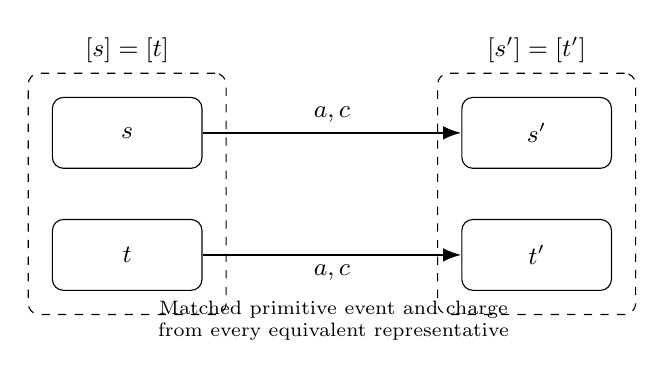
\begin{tikzpicture}[>=Latex,font=\small,b/.style={draw,rounded corners,align=center,minimum width=19mm,minimum height=9mm}]
\node[b] (s) at (0,0) {$s$}; \node[b] (t) at (0,-1.55) {$t$};
\node[draw,dashed,rounded corners,fit=(s)(t),inner sep=3mm,label={[font=\small]above:{$[s]=[t]$}}] {};
\node[b] (sp) at (5.2,0) {$s'$}; \node[b] (tp) at (5.2,-1.55) {$t'$};
\node[draw,dashed,rounded corners,fit=(sp)(tp),inner sep=3mm,label={[font=\small]above:{$[s']=[t']$}}] {};
\draw[->,thick] (s.east)--node[above]{$a,c$}(sp.west);
\draw[->,thick] (t.east)--node[below]{$a,c$}(tp.west);
\node[align=center,font=\scriptsize] at (2.62,-2.38) {Matched primitive event and charge\\from every equivalent representative};
\end{tikzpicture}
\caption{A path lifts from \emph{any} representative only under a matching-transition hypothesis; projecting concrete edges to classes alone is weaker.}
\label{fig:matching}
\end{figure}

\paragraph{Why the joint hypothesis cannot be omitted.} A quotient formed only by projecting all original edges can introduce a spurious mixed path: its first step may arrive at a class through one representative while its second step is available only from a different representative. A weaker abstraction remains safe for the one-way statement ``abstractly unreachable implies concretely unreachable,'' but not for exact reachability or path costs. Likewise, an equivalence relation preserving only settlement need not preserve proof witnesses; and blindly intersecting independently proposed nondeterministic bisimulations need not preserve the matching property. The joint relation itself must be checked.

\section{A finite quotient, and the spurious path it prevents}\label{sec:finite-case}
A quotient theorem is easier to appreciate when one sees both a legal compression and the precise failure of an illegal one. The next models are finite, so their classes and matching conditions can be inspected exhaustively. They are illustrative proof-search graphs, not reported AMLD+0 executions.

\begin{example}[An exact audit-and-cost quotient]\label{ex:finite-positive}
Let $S=\{z,u,v,t_u,t_v\}$, with exactly the four edges
\[
 z\xrightarrow{a,2}u,\qquad z\xrightarrow{b,3}v,
 \qquad u\xrightarrow{c,1}t_u,\qquad v\xrightarrow{c,1}t_v.
\]
The target is $T=\{t_u,t_v\}$. Set $q(z)=\mathsf{start}$, $q(u)=q(v)=\mathsf{pending}$, and $q(t_u)=q(t_v)=\mathsf{proved}$. Let $\sim$ have the three classes $\{z\}$, $\{u,v\}$, $\{t_u,t_v\}$. The only nontrivial matching check is between $u$ and $v$: both have precisely one $c$-edge of cost $1$ to equivalent target states. Target status and audits agree within classes. Therefore Theorem \ref{thm:joint} applies. The quotient retains exactly the target-reaching labeled-cost traces $(a,2),(c,1)$ and $(b,3),(c,1)$ from $z$; their primitive costs are respectively $3$ and $4$, and the minimum is $3$. The quotient uses three state classes rather than five states. Nothing here proves a reduction of end-to-end search cost.
\end{example}

\begin{example}[A tempting but invalid class merge]\label{ex:finite-negative}
For the negative graph use the reachable states $S^{-}=\{z,u,v,t_v\}$, retaining the two starting edges but only the $v\xrightarrow{c,1}t_v$ exit. The target is now $T^{-}=\{t_v\}$. The two non-target states $u$ and $v$ still have the same current audit $\mathsf{pending}$, yet cannot be joined by a matching-transition bisimulation. The existential quotient would nevertheless include an edge $[u]=[v]\xrightarrow{c,1}[t_v]$, producing an abstract path $(a,2),(c,1)$ from $z$ that does not exist concretely. Starting specifically at $u$, the quotient falsely advertises target reachability. The original graph can still reach a target along the $b,c$ branch, showing why a globally correct yes/no answer from $z$ would not excuse the spurious labeled path or the unsound claim about $u$.
\end{example}

\begin{figure}[htbp]\centering
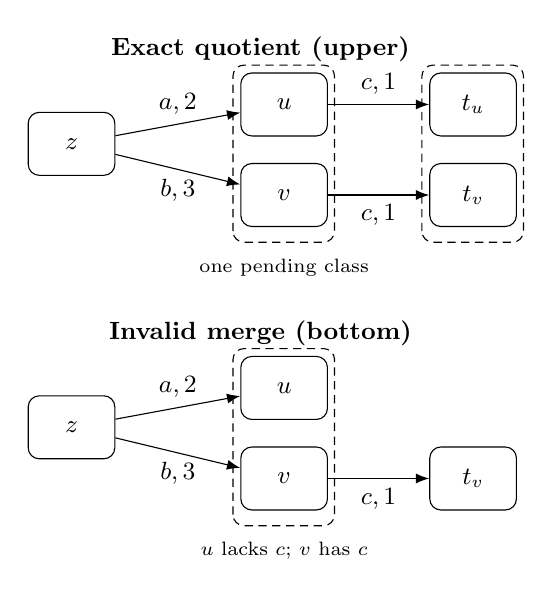
\begin{tikzpicture}[>=Latex,font=\small,ns/.style={draw,rounded corners,minimum width=11mm,minimum height=8mm,inner sep=2pt}]
\node[font=\small\bfseries] at (-2.8,2.05) {Exact quotient (upper)};
\node[ns] (z) at (-5.2,.85) {$z$};
\node[ns] (u) at (-2.5,1.35) {$u$};\node[ns] (v) at (-2.5,.20) {$v$};
\node[ns] (tu) at (-.1,1.35) {$t_u$};\node[ns] (tv) at (-.1,.20) {$t_v$};
\draw[->] (z)--node[above]{$a,2$}(u);\draw[->] (z)--node[below]{$b,3$}(v);
\draw[->] (u)--node[above]{$c,1$}(tu);\draw[->] (v)--node[below]{$c,1$}(tv);
\draw[densely dashed,rounded corners] (-3.15,-.4) rectangle (-1.86,1.85);
\draw[densely dashed,rounded corners] (-.75,-.4) rectangle (.54,1.85);
\node[font=\scriptsize,align=center] at (-2.5,-.72) {one pending class};
\begin{scope}[yshift=-3.6cm]
\node[font=\small\bfseries] at (-2.8,2.05) {Invalid merge (bottom)};
\node[ns] (zz) at (-5.2,.85) {$z$};
\node[ns] (uu) at (-2.5,1.35) {$u$};\node[ns] (vv) at (-2.5,.20) {$v$};
\node[ns] (tt) at (-.1,.20) {$t_v$};
\draw[->] (zz)--node[above]{$a,2$}(uu);\draw[->] (zz)--node[below]{$b,3$}(vv);
\draw[->] (vv)--node[below]{$c,1$}(tt);
\draw[densely dashed,rounded corners] (-3.15,-.4) rectangle (-1.86,1.85);
\node[font=\scriptsize,align=center] at (-2.5,-.72) {$u$ lacks $c$; $v$ has $c$};
\end{scope}
\end{tikzpicture}
\caption{The upper quotient is justified because the two pending states match each other's labeled, costed successors. In the lower graph the same class merge would fabricate an $a,c$ trace: one representative cannot execute the other's $c$-step.}
\label{fig:finite-example}
\end{figure}

\paragraph{Relation to the evidence ledger.} The finite example preserves the specified state audit $q$. It becomes an epistemic quotient for execution histories only when endpoint compatibility $Q=q\circ e$ is established, and a claim about proof-certificate reconstruction still needs the separate verifier and provenance interfaces. The example therefore illustrates, rather than silently assumes, the extra obligations of the combined theory.

\section{The effectiveness boundary for future memory}
A mathematically defined prospective quotient need not have a terminating general membership test, even when every finite individual audit and transition step is computable. We prove this using an elementary bounded-simulation example; it is not an implementation claim about the original oracle protocol.

\begin{theorem}[Undecidability of prospective equivalence in a computable system]\label{thm:undec}
There exists a deterministic audit transition system with finitely encoded states, a computable $\{0,1\}$-valued audit $Q$, and a total computable transition function for its single action, such that no total computable procedure decides whether two presented states are future-observationally equivalent.
\end{theorem}
\begin{proof}
Let the system have states $s_{e,k}$, for each machine/input code $e$ and $k\in\N$, together with one state $z$. Its only action is $a$, and let
\[
\delta(s_{e,k},a)=s_{e,k+1},\qquad \delta(z,a)=z.
\]
Set $Q(z)=0$ and
\[
Q(s_{e,k})=\begin{cases}
1,&\text{if the machine coded by $e$ halts within $k$ simulated steps},\\
0,&\text{otherwise.}
\end{cases}
\]
The transition and each audit value are computable by finite operations. From $s_{e,0}$, the sequence of audit outputs is identically zero exactly when the machine coded by $e$ never halts (using the standard zero-step convention). Since every audit from $z$ is zero, $s_{e,0}\equiv_{Q,\delta}^{+}z$ if and only if $e$ never halts. A total decision procedure for this equivalence would decide nonhalting and therefore halting on arbitrary inputs, contradicting the standard diagonal halting argument.
\end{proof}

\begin{remark}[What does and does not follow]
Theorem \ref{thm:undec} says a universal algorithm for the coarsest future quotient is impossible across all computable audit transition systems. It does \emph{not} rule out decidable future equivalence for particular finite-state or suitably restricted protocols, and it does not imply that the inherited oracle-ledger model contains this exact abstract subsystem. It shows why an extensional existence theorem must not be advertised as an effective compression algorithm without further structural hypotheses.
\end{remark}

\section{Source deactivation, horizons, and semantic limits}
\begin{proposition}[Closed-history survival: abstract and effective forms]\label{prop:oracle}
Assume the successful source-to-relay handoff, durability, successful post-deactivation delivery, source-independent validation, and locally closed receiver storage stipulated in A and B. Once an admissible receiver history $h$ is installed, a $Q$-sufficient retention $R(h)$ admits a \emph{mathematically defined} reconstruction of the chosen retrospective audit without using a new oracle answer. The Pioneer can \emph{execute} that reconstruction from its retained representation only if the decoder is computable on all required reachable states (for instance, by Proposition \ref{prop:effective} under its enumeration hypotheses, or by an explicit decoder). For an effectively continuing Pioneer, the prospective criterion of Theorem \ref{thm:dynamic} must additionally hold and its induced audit, enabledness, and update operations must be computable as specified in Definition \ref{def:effective}.
\end{proposition}
\begin{proof}
The inherited handoff hypotheses establish a finite locally closed history without a new oracle query. Theorem \ref{thm:static} yields a well-defined set-theoretic decoder on the image of $R$, but the construction by choosing a preimage does not itself give an algorithm. Effectiveness follows only from an additional effective-decoding hypothesis; Example \ref{ex:truth-obstruction} shows why this cannot be omitted for a truthful-oracle family. Theorem \ref{thm:dynamic} separately gives the extensional prospective criterion. Its abstract quotient operations are executable only when there are algorithms for decoding, enabledness, and updates, as the restricted construction in Example \ref{ex:concrete-ledger} demonstrates.
\end{proof}

For the one-drop horizon inherited from Completions A and B, first normalize each machine code $e$ by inserting one dummy simulated step before its original computation can halt. Write $\widehat e$ for this effective normalization; it does not change whether the machine ever halts. Define
\[
h_e(k)=\begin{cases}2,&\widehat e\text{ has not halted in its first $k$ simulated steps},\\1,&\widehat e\text{ has halted by step $k$}.\end{cases}
\]
Each $h_e(k)$ is computable by bounded simulation, each sequence is nonincreasing, and $h_e(0)=2$. Put
\[
F(e,N)\iff \forall k\ge N\ [h_e(k)=h_e(N)].
\]
The predicate $F$ has the Turing degree of the halting problem. Indeed, for every pair $(e,N)$ one can effectively generate a machine $m_{e,N}$ that computes $h_e(N)$ and halts if and only if it later discovers some $k>N$ with $h_e(k)\ne h_e(N)$. Thus $F(e,N)\iff H(m_{e,N})=0$, showing $F\le_T H$. Conversely the dummy-step normalization ensures $F(e,0)$ is true exactly when $e$ never halts, giving $H\le_T F$ by negating that answer. Without the dummy-step convention, the converse as phrased could fail for a machine halting at stage zero; the normalization is an essential hypothesis, not merely typographical.

No total ordinary computable selector can choose a final stabilization stage $N(e)$ for all $e$: given such a selector one could compute $h_e(N(e))$ and thereby decide halting, contrary to the diagonal argument. The inherited oracle receipt grammar permits only halting-bit assertions. A separately checked effective reduction from finality to the legitimate halting-bit query for $m_{e,N}$ supports a correctly typed \emph{derived testimonial note}, not a native source attestation of $F(e,N)$ and not a $V$-accepted proof of finality.

\begin{proposition}[Finite preserved answers do not yield universal oracle power]
Any fixed finite, source-deactivated archive of oracle-answer bits can be hard-coded as a finite constant in an otherwise computable procedure. It does not, solely by being preserved or losslessly re-encoded, make that procedure a total decider for the halting predicate on all inputs.
\end{proposition}
\begin{proof}
If a uniform computable algorithm with that fixed finite archive decided halting on all inputs, hard-code the same finite archive into its program. This yields an ordinary total computable halting decider, contradicting the diagonal argument. Exact compression or decompression of a fixed finite archive changes no part of this reasoning.
\end{proof}

The new prospective-undecidability theorem and the inherited one-drop finality theorem have a common conceptual lesson: a finite current observation and a theorem that a final distinction exists do not imply effective recognition of every future distinction. They are not claimed to be the same predicate or to have identical implementations.

\begin{figure}[htbp]\centering
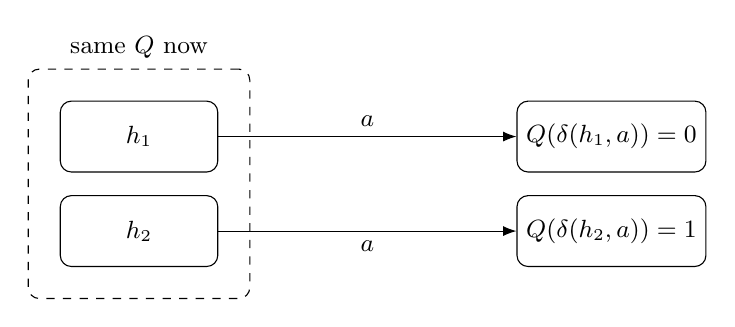
\begin{tikzpicture}[>=Latex,every node/.style={font=\small},b/.style={draw,rounded corners,minimum width=20mm,minimum height=9mm,align=center}]
\node[b] (x) at (0,0.6) {$h_1$};
\node[b] (y) at (0,-0.6) {$h_2$};
\node[draw,dashed,rounded corners,fit=(x)(y),inner sep=4mm,label=above:{same $Q$ now}] {};
\node[b] (xx) at (6,0.6) {$Q(\delta(h_1,a))=0$};
\node[b] (yy) at (6,-0.6) {$Q(\delta(h_2,a))=1$};
\draw[->] (x.east)--node[above]{$a$}(xx.west);
\draw[->] (y.east)--node[below]{$a$}(yy.west);
\end{tikzpicture}
\caption{One current audit class can contain states with different observable futures. Prospective preservation must retain the distinction.}
\label{fig:future-split}
\end{figure}

\section{Trading presentations while preserving evidence}\label{sec:trades}
Trading Theorem 003 represents a formal presentation as $P=(x,y,A,R)$, with finitary inference rules $R$, axioms $A$, and consequence closure $\operatorname{Cn}_P(\Gamma)$. Mutual contextual reproducibility of resource families $U$ and $V$ over a fixed background establishes
\[
\operatorname{Cn}_{B+U}(\Gamma)=\operatorname{Cn}_{B+V}(\Gamma)
\quad\text{for every admissible hypothesis bank }\Gamma.
\]
This is a statement about \emph{deductive power}. It can preserve whether a theorem is provable without preserving its shortest certificate, the intermediate proof-search states, the cost of checking a result, or the history by which a particular Pioneer obtained it.

\begin{example}[A theorem macro is not a full history quotient]
Suppose a lemma $\lambda$ has an accepted primitive derivation $\pi$. A verified macro can make $\lambda$ available by a shorter reference while retaining $\pi$ for checking. The conclusion and theoremhood are unchanged. But the primitive expansion, the macro's stored address, and the record of who discovered $\pi$ are different potential evidence objects. Trading Theorem 003 explicitly separates compressed macro cost from fully expanded primitive-certificate cost. A quotient based only on the consequence class may therefore be valid for theoremhood and invalid for a full provenance audit.
\end{example}

A safe synthesis proposes three independent proof obligations for a candidate trade: \emph{consequence preservation} (via contextual simulation or a suitable checked translation), \emph{audit preservation} (via Theorem \ref{thm:static} or \ref{thm:endpoint}), and \emph{transition/trace preservation} (via Theorem \ref{thm:joint} or an appropriately weaker one-way simulation). None of these is silently inferred from the other two.

\section{What the quotient does not promise: fully charged cost}\label{sec:economics}
It is important to distinguish three uses of ``compression'': (1) a partition into fewer observational or settlement classes, (2) a short code for a retained state or a certificate, and (3) a decrease in the cost of actually discovering a verified settlement. Theorems \ref{thm:bits} and \ref{thm:joint} concern (1) and limited aspects of (2); they do not prove (3).

For a frozen ATP, target family and task distribution, a declared accounting model could separately charge
\begin{align*}
C_{\rm total}={}&C_{\rm quotient\,build}+C_{\rm check\,invariants}+C_{\rm class\,lookup}\\
&+C_{\rm search}+C_{\rm lift}+C_{\rm witness\,restore}+C_{\rm verify}+C_{\rm scheduling}.
\end{align*}
This is a proposed ledger of cost categories rather than a universal equality across physical machines. Primitive path costs are not the same quantity as $C_{\rm total}$; even equality of all primitive target-path traces permits very different quotient discovery, lookup and verification work. A theorem requiring an ideal $H$-oracle does not imply a finite-cost executable oracle service. A cardinality lower bound on storage bits is not a bound on CPU time, circuit size, or total persistent memory including decoder and provenance tables.

\begin{figure}[htbp]\centering
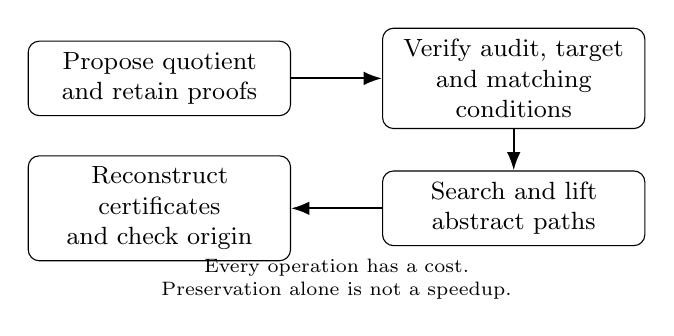
\begin{tikzpicture}[>=Latex,font=\small,b/.style={draw,rounded corners,align=center,minimum height=9mm,inner sep=4pt}]
\node[b,text width=3.05cm] (p) at (0,0) {Propose quotient\\and retain proofs};
\node[b,text width=3.05cm] (v) at (4.5,0) {Verify audit, target\\and matching conditions};
\node[b,text width=3.05cm] (l) at (4.5,-1.65) {Search and lift\\abstract paths};
\node[b,text width=3.05cm] (c) at (0,-1.65) {Reconstruct certificates\\and check origin};
\draw[->,thick] (p)--(v);\draw[->,thick] (v)--(l);\draw[->,thick] (l)--(c);
\node[align=center,font=\scriptsize] at (2.25,-2.55) {Every operation has a cost.\\Preservation alone is not a speedup.};
\end{tikzpicture}
\caption{A quotient can reduce the number of stored classes while increasing the work required to validate and exploit the representation.}
\label{fig:charged}
\end{figure}

\paragraph{A feasible restricted project.} On a finite effectively represented transition system with a finite set of labeled edges and decidable audit and target predicates, a specified candidate state-equivalence relation can be checked by exhaustive enumeration for the conditions of Theorem \ref{thm:joint}. The existence of a \emph{useful} candidate, however, and the cost of checking candidates are separate questions. Such a finite prototype would be an appropriate setting for an experimentally measured Quotient Hunter; it would not settle the undecidability barrier for general infinite systems.

\section{A unified hierarchy of obligations and open problems}
The combined framework permits an orderly sequence of checks without implying that every stage can be completed algorithmically.
\begin{enumerate}[label=\arabic*.]
\item \textbf{Choose the audit.} Record whether the Pioneer promises a Boolean admission flag, a typed evidence vector, complete certificate bytes, or auditable origins. These are different mathematical interfaces.
\item \textbf{Choose the state and history models.} Say whether the transition system distinguishes receipt IDs, queue and budget states, and random or environmental events. Use exact history addresses when preserving occurrence identity is required.
\item \textbf{Test endpoint sufficiency.} If the audit cannot factor through the final state, do not quotient that state further and claim the lost audit survived.
\item \textbf{Test future behavior.} For deterministic actions, require an audit-preserving transition congruence; for branching proof search, check the combined two-way label-and-cost matching hypotheses when exact target traces are advertised.
\item \textbf{Keep proof and origin interfaces typed.} Verifier approval of a proof DAG is not certification that a particular execution created that DAG. Translate and independently check each claim at the appropriate gate.
\item \textbf{Account for computability and total cost.} Identify executable decoders and lifts before promising operational continuation, then measure full search and checking charges against an unchanged baseline.
\end{enumerate}

\begin{conjecture}[Cost-sensitive certified quotient discovery]
There exist nontrivial constrained families of verifier-gated proof-search systems for which an effectively found joint audit--settlement quotient preserves a declared nontrivial provenance interface and lowers a fixed, fully charged discovery-cost objective relative to an agreed unquotiented baseline. This is not asserted for every system, target, or cost model.
\end{conjecture}

\begin{conjecture}[Effective restricted future equivalence]
Some useful effectively presented infinite-state protocol families may admit finite symbolic criteria for future-observational equivalence and computable canonicalization. The general undecidability theorem for computable audit transitions does not preclude such restricted positive results, but no universal algorithm follows.
\end{conjecture}

The strongest practical research objective is not ``store the theorem'' and not ``remember everything.'' It is \emph{retain exactly the distinctions demanded by the declared audit and the promised continuation and proof-verification interfaces}. This objective is a mathematics of preservation, not a guarantee that a globally optimal representation exists or is computable.

\section{Conclusion and verification ledger}
Completion C's conservation theorem explains when a smaller archive can answer the same authorized historical questions. The geometry of Exact Addressing explains why a history, its final state, and an extracted accepted proof are not interchangeable. The Trading Theorem contributes the possibility of changing deductive presentations or collapsing search states without changing settlement. The joint quotient theorem connects these ideas by placing audit and settlement under one transition-matching hypothesis, then separating abstract preservation from executable lifting and from proof-origin certification.

The overarching implication is \emph{conditional}: if an ATP has a suitable exact representation and a verified quotient with the required typed interfaces, it can forget certain details without forfeiting specified mathematical capabilities or claims about its evidence. What those details are depends on the interface. Even when the best abstract partition exists, recognizing its classes can be undecidable; even when it is computable, finding and using it may cost more than it saves.

\begin{center}\small
\begin{tabular}{@{}p{0.41\linewidth}p{0.51\linewidth}@{}}\toprule
\textbf{Mathematical obligation}&\textbf{Status in this integrated article}\\\midrule
Evidence types and verifier firewall&Inherited frozen conditional calculus from Completions A/B/C\\
Exact retrospective preservation and bit lower bound&Paper-level proofs retained from Completion C\\
Abstract versus computable decoding&Counterexample and effective sufficiency conditions retained from Completion C\\
History unfolding and typed extraction&Exact Addressing P.1/P.3 argument restated with conditions\\
Endpoint audit factorization&Theorem \ref{thm:endpoint}, derived from static preservation\\
Restricted continuing ledger&Explicit two-bit construction and one-bit obstruction\\
Prospective observational equivalence&Proofs and undecidability result retained from Completion C\\
Joint audit--settlement weighted quotient&Re-audited Theorem \ref{thm:joint}; exact audit-annotated traces\\
Finite example and spurious-path test&Examples \ref{ex:finite-positive}--\ref{ex:finite-negative}, fully specified\\
Executable path lifting and origin certificates&Additional declared algorithm/checker interfaces required\\
General compression optimality, cost reduction, proof assistant check&Not established or performed\\\bottomrule
\end{tabular}
\end{center}
\clearpage
\section*{Provenance and references}\addcontentsline{toc}{section}{Provenance and references}
\noindent\textbf{Direct supplied mathematical sources.} \texttt{<Brian Tenneson>}, \emph{Completion C: The Epistemic Conservation of Mathematical Histories}, ATLAS-repaired version 0.2, October 30, 2026 (published separately in the author's \texttt{pub} library); \texttt{<Brian Tenneson>}, \emph{After Completion C: Certified Quotient Geometry of Mathematical Histories}, expository 0.1; \texttt{<Brian Tenneson>}, \emph{Trading Theorem 003: Mutual Reproducibility, Consequence-Preserving Trades, Quotient Hunting, and Verified Settlement Search}, September 17, 2026; and \texttt{<Brian Tenneson>}, \emph{Exact Addressing 4.14, Prologue: The Structure and Geometry of Automated Theorem Proving}, preliminary release. The completed Level-1 A/B papers were consulted through their retained texts and their descendants in Completion C. The founding seven-page Oracle-Attested Mathematical Knowledge note ($W_0$) remains an identified immutable ancestor. No paper listed in the Trading Theorem's external bibliography was separately consulted for this synthesis.\\[5pt]
\noindent\textbf{ATLAS repair record.} Relative to integrated version 0.1, version 0.2 (i) makes execution histories and accepted evidence snapshots explicitly different types and specifies their readout, (ii) states audit-trace preservation in the joint bisimulation result, (iii) introduces paired finite exact/invalid quotient examples, and (iv) repairs the one-drop nonhalting reduction by an effective dummy-step normalization. These changes do not install a verifier or constitute independent peer review.\\[5pt]
\noindent\textbf{New manuscript identity.} The current manuscript is an integrated successor, not a revision or replacement of the published Completion C and not an append-only bundle of the two most recent manuscripts. The quoted or adapted mathematical results have been reorganized for continuous exposition, and the endpoint and joint quotient statements are explicitly marked as derived syntheses. No source PDF, LaTeX ancestor, repository entry, or ATP executable was modified in making this file. The diagrams are original expository schematics, not proof certificates.

\section*{Disclaimer on Mathematical Accuracy, Authorship, and Artificial Intelligence}\addcontentsline{toc}{section}{Disclaimer on Mathematical Accuracy, Authorship, and Artificial Intelligence}
Every reasonable effort has been made to ensure that the mathematical exposition presented herein is factual, correct, logically sound, sufficiently complete in its treatment of relevant facts (not in the technical sense of G\"odelian completeness), and supported by rigorous proofs or, at minimum, not readily susceptible to refutation. Nevertheless, no guarantee of correctness, completeness, consistency, or provability is implied. The authorship and composition of this work involve a combination of human and artificial intelligence. DATA MIND (OpenAI GPT-6), operating under the direction and mathematical research program of \texttt{<Brian Tenneson>}, assisted in developing mathematical statements, organizing proofs, choosing exposition, and preparing the manuscript. This ATLAS-repaired integrated successor preserves the distinction between abstract and executable reconstruction, incorporates restricted continuing-ledger and finite weighted-quotient examples, and adds conditional quotient-preservation arguments. Such assistance is not a substitute for independent mathematical verification. Formal proof-assistant checking, independent refereeing, operational AMLD+0 settlement, and physical validation of a noncomputable oracle were not performed. Statements labeled as conjectures remain unproved; all preservation, effectiveness, and soundness conclusions are limited by their expressly stated hypotheses. This draft is not evidence that a computational engine or protocol has been installed or altered. It is unpublished; the earlier publication of Completion C is not an authorization to publish this successor.
\end{document}
